\chapter{Wstęp teoretyczny}
\label{cha:wstepTeoretyczny}

%---------------------------------------------------------------------------

\section{Procesy biznesowe}
\label{sec:procesyBiznesowe}

\subsection{Procesy biznesowe}
W każdym dużym przedsiębiorstwie, każdego dnia, wykonywana jest ogromna ilość czynności koniecznych do funkcjonowania tej organizacji. Ludzie oraz systemy podejmują najróżniejsze działania związane z różnymi, często nie mającymi wiele wspólnego zadaniami jak chociażby procesowanie płatności, składnie zamówień, wytwarzanie produktów czy ich transport. Przykłady te można mnożyć w zależności od sektora w jakim obraca się dana firma. Im jest ona większa, tym trudniej jest osobom zarządzającym zrozumieć i opisać poszczególne czynności. W pewnym momencie, kiedy ilość rożnych zadań rośnie do setek czy tysięcy staje się to niemożliwe i potrzebny jest sposób na zebranie wiedzy o pojedynczych operacjach i zamknięcie ich w uporządkowaną strukturę. Stąd narodził się pomysł na wykorzystanie wykorzystanie procesów biznesowych.

Procesy biznesowe opisują zbiór aktywność, które podejmuje grupa podmiotów w celu osiągnięcia celu biznesowego. W literaturze brakuje jednej ogólnie przyjętej definicji procesu biznesowego. W latach 90. XX wieku proponenci BPR, czyli Przeprojektowania procesów biznesowych (\textit{eng. Business process re-engineering}) starali się sprecyzować pojęcie procesu biznesowego. W książce ,,Process Innovation: Reengineering Work through Information Technology''\cite{davenport1993process} określono termin ten jako ,,Ustrukturyzowany, mierzalny zbiór działań, których celem jest wytworzenie określonego produktu dla określonego klienta lub rynku''. Autor położył nacisk na zbiór kroków prowadzących do celu, raczej niż na końcowy efekt. W dalszej części autor pisze ,,Proces jest zatem określonym uporządkowaniem czynności roboczych w czasie i przestrzeni, z początkiem i końcem oraz jasno określonymi wejściami i wyjściami: strukturą działania.''. Inni pionierzy BPR Michael Hammer i James Champy zaproponowali  podejście ,,Proces biznesowy to zbiór działań, który pobiera jeden lub więcej rodzajów danych wejściowych i tworzy wynik, który ma wartość dla klienta''\cite{HAMMER199390}. Autorzy dają większą dowolność, co do definicji procesu, nie wspominając o konieczności jego logicznej organizacji czy mierzalności. Z kolei Jacobson zupełnie pomija konieczność zamknięcia procesu w jakiekolwiek ramy: ,,Zestaw czynności wewnętrznych wykonywanych w celu obsługi klienta''\cite{JacobsonObjectAdvantage}. Nacisk na konieczność odniesienia procesów do wymiernych środków firmy widzimy w definicji: ,,Procesy biznesowe są aktywną częścią biznesu. Opisują funkcje firmy i obejmują zasoby, które są używane, przekształcane lub wytwarzane. Proces biznesowy to abstrakcja, która pokazuje współpracę między zasobami i transformację zasobów w biznesie. Podkreśla, w jaki sposób wykonywana jest praca, zamiast opisywać produkty lub usługi wynikające z tego procesu.''\cite{Eriksson2000BusinessMW}. Szczególnie ważny jest tutaj fragment o transformacji zasobów, gdyż każe on rozumieć poszczególne aktywności w procesie jako powiązane ze sobą i kończące się namacalnymi rezultatami. Definicja ,,Proces biznesowy to seria kroków mających na celu wytworzenie produktu lub usługi. W wyniku niektórych procesów produkt lub usługa jest odbierana przez zewnętrznego klienta organizacji. Nazywamy te podstawowe procesy. Inne procesy wytwarzają produkty, które są niewidoczne dla klienta zewnętrznego, ale są niezbędne do efektywnego zarządzania firmą. Nazywamy te procesy wsparcia''\cite{rummler_brache_1995} wprowadza rozgraniczenie na podtypy procesów. Ważnym jest jednak że nie jest koniecznością, aby rezultaty procesu były widoczne na zewnątrz organizacji. Warto też zaznaczyć, że procesy biznesowe nie dotyczą jednej osoby czy nawet działu, a raczej udział w nich bierze wiele ludzi, maszyn czy systemów z różnych działów połączonych celem dostarczenia wspólnej wartości biznesowej.

Powyższe definicji skupiają się na delikatnie odmiennych aspektach procesów biznesowych, nie zawsze szczegółowo wspominając o innych. Starając się usystematyzować powyższe sformułowania, chcąc zbudować bazę do dalszej analizy tematu, można przyjąć, że procesy biznesowe charakteryzują:
\begin{itemize}
  \item[•] Określony cel, którym jest wytworzenie wartości dla klienta zewnętrznego lub pośrednio firmy - klienta wewnętrznego. Jednak warto jeszcze raz zaznaczyć ze proces biznesowy skupia się na sposobie osiągnięcia celu, a nie opisie celu samego w sobie. 
  \item[•] Dyskretny, jasno zdefiniowany i identyfikowalny zbiór aktywności. 
  \item[•] Jasno określony początek - wejście i koniec - wyjście.
  \item[•] Zależność przyczynowo-skutkowa pomiędzy kolejnymi procesami.
\end{itemize}

Żeby lepiej zilustrować czym jest proces biznesowy, poniżej znajduje się prosty przykład często spotykanego procesu. Oczywiście, prawdziwy proces będzie składał się z o wiele większej liczby aktywności.

\begin{figure}[h]
	\centering{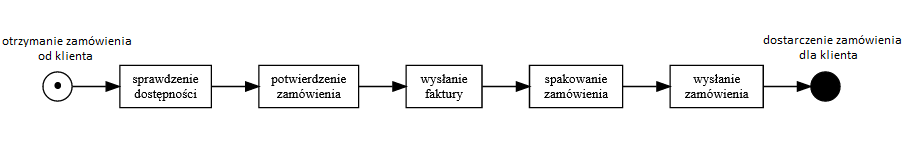
\includegraphics[scale=0.7]{simple-business-process.png}}
	\caption{\label{fig:simple_business_process}Przykład prostego procesu}
\end{figure}

Zauważmy, że mamy jasno zdefiniowany wejście - otrzymanie zamówienia od klienta oraz wyjście, kiedy dostarczamy oczekiwaną wartość dla klienta, a całość składa się z serii tworzących logiczną całość aktywności. Aktywności są konkretnie zdefiniowane. Standardem jest definiowanie aktywności w formie równoważników zdań.


\subsection{Zarządzanie procesami biznesowymi}
Zdefiniowanie proces biznesowego otwiera wiele możliwości analizy działań przedsiębiorstwa i w skutek tego wprowadzanie usprawnień. Dziedziną, która się tym zajmuje jest zarządzanie procesami biznesowymi (\textit{eng. Business process modeling}) zwane w skrócie BPM. Sercem jest proces, a samo BPM jest dyscypliną używającą różne metody, technik i sposobów w celu projektowania, wprowadzania w życie, zarządzania i analizy procesów biznesowych \cite{BPMDemystified}. 

Celem stosowania metod zarządzanie procesami biznesowym jest udoskonalanie procesów w danej organizacji biznesowej. Udoskonalanie może być rozumiane jako w różnoraki sposób w zależności od kierunku rozwoju firmy. Może to być na przykład redukcja czasu, kosztów, czy dostarczanie lepszego produktu końcowy. Ważnym jest aby było to podejście całościowe i odnosiło się do całego zbioru aktywności w ramach danego procesu. Usprawnianie pojedynczej aktywności to nie BPM. Patrząc na przykład powyżej, jeśli wprowadzilibyśmy usprawnienia w ramach wysyłania faktury, robiąc to elektronicznie zamiast tradycyjną poczta, mimo że taka zmiana przyniosłaby poprawę wydajności, nie mielibyśmy do czynienia z zarządzaniem procesami biznesowymi. O BPM moglibyśmy mówić, gdybyśmy  znaleźli sposób, żeby przeprojektować cały proces tak, żeby wysyłanie faktury nie było potrzebne lub odwrotnie, jeśli dodalibyśmy nowe aktywność, która usprawniłaby proces jako całość czy nawet zmieli kolejności zdań w procesie, gdyż zmiany w ramach poszczególnych, jednostkowych aktywności nie są konieczne, żeby ulepszyć proces jako całość \cite{BPMWhat}.

Zarządzanie procesami biznesowymi jest zbiorem praktyk, działań mających na celu udoskonalanie procesów. Trzeba więc rozumieć BPM jako pojęcie abstrakcyjne, jednak szczególnie w dzisiejszym świecie, zarządzanie procesów biznesowych nie może się obyć bez wsparcia ze oprogramowania czy technik znanych z różnych dziedzin informatyki \cite{BPMSurvey}. Na lepsze zrozumienie czym zajmuje się zarządzanie procesami biznesowymi oraz w jaki sposób możemy zastosować informatykę, a w szczególności eksplorację procesów w tej dziedzinie, może pozwolić definicja cyklu życia procesu biznesowego.

\begin{figure}[h]
	\centering{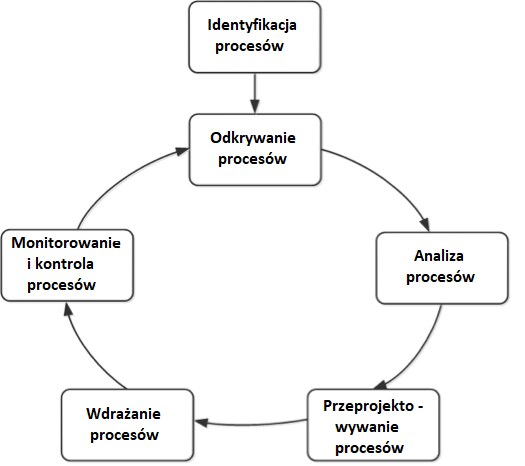
\includegraphics[scale=0.55]{lifecycle.png}}
	\caption{\label{fig:lifecycle}Cykl życia procesu biznesowego}
\end{figure}

Cykl życia procesu biznesowego (\textit{eng. Business process lifecycle}) przedstawiono na rys. \ref{fig:lifecycle} \cite{dumas2013fundamentals}. Jest to zbiór kroków niezbędnych do skutecznego zarządzania procesami biznesowymi. W celu dostosowania do zmieniającej się rzeczywistości, poszczególne kroki powinny być co pewien czas powtarzane. 

Konieczność powtarzania elementów cyklu życia procesu biznesowego sygnalizuje przewagę komputerów i algorytmów nad wykonywaniem tych operacji przez człowieka. Metody informatyczne są stosowane, na każdym z wymienionych etapów. W szczególności dane zebrane w wyniku monitorowania procesów dają nam możliwość zastosowania metod z zakresu eksploracji procesów (sekcja \ref{sec:eksploracja}). Praca skupia się w głównej mierze na odkrywaniu procesów, czyli znajdowaniu istniejących już procesów na podstawie realny danych. Należy zaznaczyć, że identyfikacja polega na ogólnym rozpoznaniu i nazwaniu zachodzących procesów, podczas gdy odkrywanie jest bardziej szczegółowe, a w jego wyniku otrzymujemy dokładny model.  

%---------------------------------------------------------------------------

\section{Eksploracja procesów}
\label{sec:eksploracja}
\subsection{Modelowanie procesów biznesowych}
Na rys. \ref{fig:simple_business_process} przedstawiono przykład uproszczonego procesu biznesowego. Łatwo sobie wyobrazić, że proces ten w rzeczywistości może być znacznie bardziej skomplikowany. Część aktywności może być wykonywana równolegle, niektóre zdarzenia w ogóle nie zaistnieją lub będą występować kilkukrotnie w ramach jednego procesu. 


W sytuacji, w której zamówiony przez klienta towar będzie niedostępny, logiczne wydaje się poinformowanie go o opóźnieniu oraz danie mu możliwości anulowanie zamówienia lub jego kontynuacja i ponowne sprawdzenie dostępności. Ponadto, czynności takie jak wysłanie faktury oraz spakowanie i wysłanie zamówienia mogą być wykonane w dowolnej kolejności czy nawet jednocześnie przez dwie różne osoby. Proces staje się bardziej skomplikowany i konieczna do stworzenia jego modelu jest bardziej złożona notacja niż użyta do przedstawienia prostego procesu. 
Istnieje wiele notacji do modelowania procesów biznesowych, wśród nich można wymienić schematy blokowe, diagramy aktywności UML, łańcuchy procesu sterowanego zdarzeniami (\textit{eng. Event-driven Process Chains}), sieci Petriego \cite{BPMComparission}. Obecnie najpopularniejszą notacją używaną do opisu procesów biznesowych jest Business Process  Model and Notation, w skrócie BPMN \cite{omg2011bpmn}. Daje ona możliwość opisania w jednoznaczny sposób skomplikowanych procesów czy stworzenia diagramów współdziałania procesów, jednocześnie pozostając łatwą do zrozumienia.

Na grafice poniżej przedstawiono notację opartą o elementy BPMN, używaną w dalszej części pracy. Składają się na nią zdarzenia początkowe i końcowe, połączenia, bramki logiczne oraz aktywności, gdzie czarnym kwadratem oznaczono sytuację, w której żadna aktywność nie jest wykonywana, możliwe tylko w bramce LUB. 
\clearpage
\begin{figure}[h]
	\centering{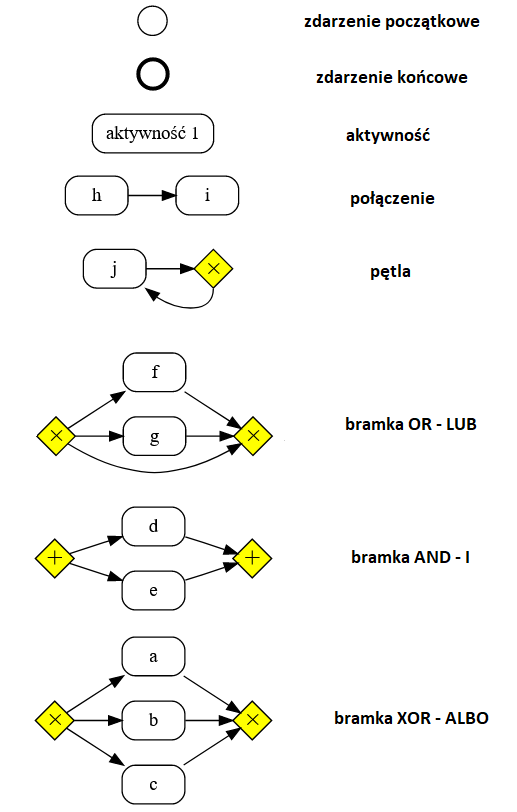
\includegraphics[scale=0.41]{BPMNelements.png}}
	\caption{\label{fig:bpmn_example}Elementy BPMN}
	\label{fig:lifecycle}
\end{figure}

Korzystając z tej notacji, można przedstawić opisany wcześniej proces. Na rys.  \ref{fig:complicated_business_process_1} widać model po modyfikacjach. 

\begin{figure}[h]
	\centering{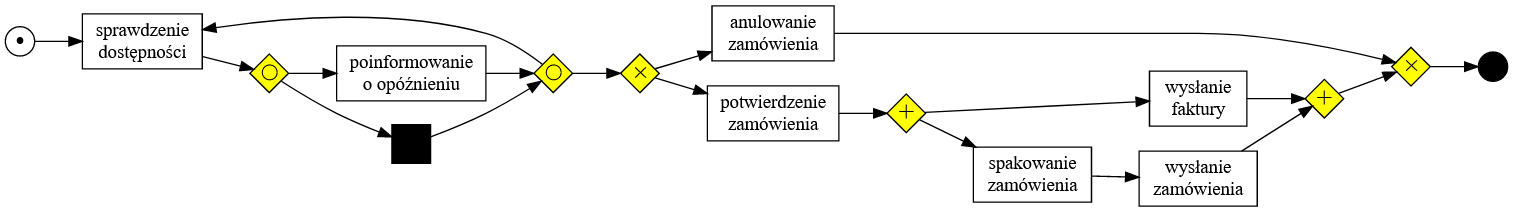
\includegraphics[scale=0.3]{complicated-process-example-1.png}}
	\caption{\label{fig:complicated_business_process_1}Rozbudowany model procesu - przykład 1}
\end{figure}

Możliwe jest teraz poinformowanie klienta o opóźnieniu, a następnie anulowanie zamówienia lub powtórne sprawdzenie dostępności. Model ten jednak nie jest wystarczająco precyzyjny i pozwala na potwierdzenie zamówienia po informacji o jego opóźnieniu, a bez uprzedniego ponownego sprawdzenia dostępności. Można zaproponować inny model (rys. \ref{fig:complicated_business_process_2}), który rozwiązuje powyższe problemy, jednak aktywność - poinformowanie o opóźnieniu - występuje na nim dwukrotnie, co jest niepożądane i  pogarsza jego czytelność.

\begin{figure}[h]
	\centering{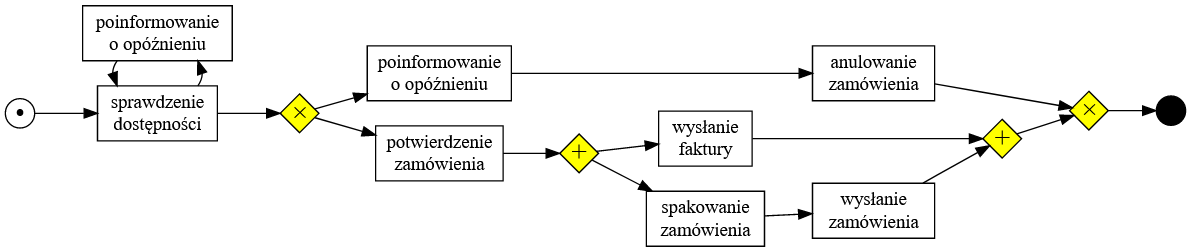
\includegraphics[scale=0.35]{complicated-process-example-2.png}}
	\caption{\label{fig:complicated_business_process_2}Rozbudowany model procesu - przykład 2}
\end{figure}

Ponadto, w pewnych przypadkach klient może mieć możliwość rezygnacji z zamówienia bez ówczesnego informowania go o opóźnieniu, a z czego nie zdawano sobie sprawy, wtedy konieczne może być stworzenie zupełnie innego modelu. Aby radzić sobie z tymi problemami powstał szereg zestawów wytycznych, którymi warto się kierować modelując procesy biznesowe. Wśród takich zasad można wymienić: zminimalizuj liczbę elementów w modelu, zminimalizuj liczbę ścieżek w modelu, używaj jednego zdarzenia początkowego i jednego końcowego, unikaj bramek LUB - OR , zdekomponuj model zawierający więcej niż 50 elementów \cite{7PMG}.

Modelowania procesów biznesowych jest próbą stworzenia uproszonej wersji rzeczywistości na podstawie przewidywań i założeń. Modele dają abstrakcję, użyteczne przybliżenie rzeczywistości, jednak należy pamiętać, że ,,Wszystkie modele są błędne'' i rzeczywisty proces najprawdopodobniej będzie różnił się od nawet najlepszego modelu. 


\subsection{Eksploracja procesów}

W dzisiejszych czasach standardem jest, że organizacje biznesowe korzystają z systemów informatycznych, takich jak chociażby systemy ERP czy CRM, wspierających ich działalność. Systemy te rejestrują dane o procesach, które wspierają. Dane te mogą być później analizowane i wykorzystane do wprowadzenie usprawnień w działaniu firmy.   

Tradycyjne metody są wolne, kosztowne i narażone na błędy ludzkie a konieczność ich ciągłego powtarzania, połączone z wszechobecnym trendem automatyzacji obecnym w biznesie sprawiają, że eksploracja procesów zyskuje na znaczeniu \cite{market-pm}. Ważna jest możliwość szybkiej adaptacji do zmian, automatyzacja pozwala na wykonywanie powtarzalny zmian i ograniczenia błędów.

Jest to szeroko pojęta dziadzina, która zawiera różne aplikacje metoda informatyki do procesów. 
Jest wartościowym dodatkiem do innych metod eksploracji danych, gdyż daje pełniejszy obraz zamiast skupiać się pojedynczym rezultacie końcowym i tworzyć predykcje, celem jest zrozumienie całej procesu i akcji, które prowadzą do końcowego rezultatu. Jest ot trudniejsze, ale jakże cenne z punktu widzenia biznesowego, gdyż jakakolwiek zmiana w trakcie procesu może sprawić, że przewidywania będą kompletnie trafione, a zrozumienie całego procesu pozwala na pełniejszy obraz i łatwiejsze dostosowanie do zmian. 

Ponadto, procesy biznesowe są często rozumiane przez analityków i metoda na łatwe odniesienie się do oczekiwań biznesowych i stworzenie ścisłych, powtarzalnych i sprawdzalnych ram na dziedzinie, która w większości opierała się na czarnej magii, bullshicie i coachingowy bredniach jest nad wyraz cenne. Eksploracja procesów biznesowych oparta jest na danych i nie ma w niej dużo miejsca na przypuszczenia i domysły.

Podsumowując, eksploracja procesów to techniki, narzędzia i
metody odkrywania, monitorowania i
usprawniania rzeczywistych procesów poprzez 
wiedzę wyodrębnioną z dzienników zdarzeń powszechnie
dostępnych w systemach informacyjnych \cite{pm-manifesto}\cite{mining-overview}.
Wyróżnia się 3 podkategorie: 
\begin{itemize}
  \item[•] automatyczne odkrywanie procesów
  \item[•] sprawdzanie zgodności (\textit{eng. conformance checking})
  \item[•] udoskonalanie procesu (\textit{eng. performance mining})
\end{itemize}


\subsection{Dzienniki zdarzeń}
\label{sec:event_logs}
Danymi wejściowymi dla algorytmów z dziedziny eksploracji procesów są dzienniki zdarzeń, inaczej zwane logami.
 
\begin{figure}[h]
	\centering{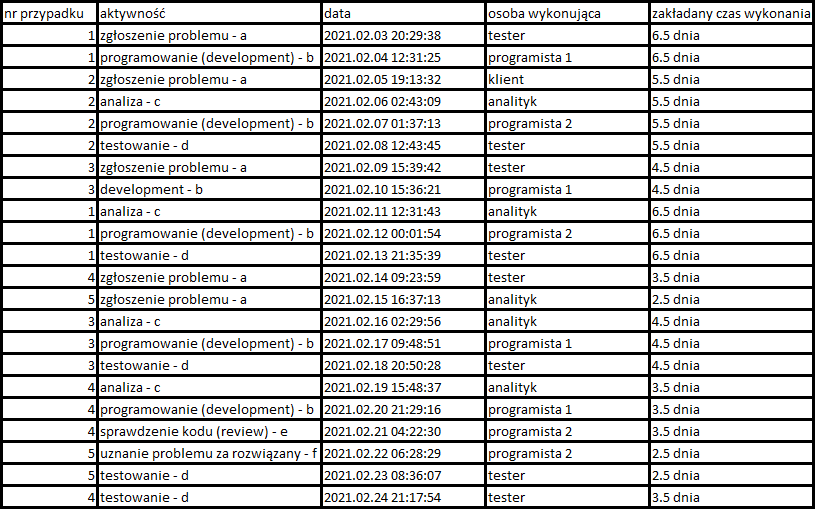
\includegraphics[scale=0.6]{event-log-example.png}}
	\caption{\label{fig:event_log_example}Przykład dziennika zdarzeń}
\end{figure}

W kontekście odkrywania procesów biznesowych ważne są dla nas tylko zdarzenia i kolejność ich wykonywania.
Przyjmuje się, że aby mówić o dzienniku zdarzeń powinien on zawierać 3 informacje: numer przypadku, czyli unikalny identyfikator zbioru aktywności, nazwę poszczególnych aktywności oraz datę jej wykonania - ważną tylko w kontekście kolejności wykonywania pojedynczych aktywności. Ponadto może on zawiera inne zbędne w kontekście odkrywania procesów biznesowych dodatkowa informacje, takie jak: podmiot wykonującym daną aktywność, miejsce, koszt czy aktualny postęp wykonania. Oczywiście te pozostałe dane mogą być wykorzystywane w kolejnych etapach analizy i usprawniania procesu.

Mając do dyspozycji te 3 informacje - poszczególne przypadki, aktywności na nie się składające oraz ich kolejność, zliczamy jak często poszczególne aktywności występują w danej kolejności. Każdy tak przypadek zwany jest wariantem. Ponadto musimy wiedzieć jak często dany wariant wystąpił.

\begin{figure}[h]
	\centering{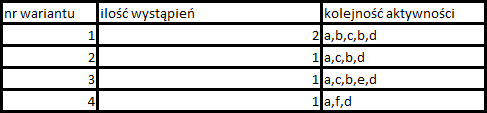
\includegraphics[scale=0.6]{variants-example.png}}
	\caption{\label{fig:process_variants_example}Przykład wariantów procesu}
\end{figure}

Dla poprawy czytelności aktywności często reprezentowane są jako symbole, np. kolejne litery alfabetu, zamiast pełnej nazwy.

\subsection{Automatyczne odkrywanie procesów biznesowych}

Automatyczne odkrywanie procesów biznesowych jest podgrupą i obejmuję techniki przekształcania danych w procesy. Ważne, że proces już istnieje, a my tylko go odkrywamy. Wejściem jest dziennik zdarzeń, a wyjściem jest mapa procesu lub model procesu.

Procesy zaprojektowane nie zawsze są realizowane w praktyce. Ważne jest, żeby proces był oparte tam analizie prawdziwych danych, a nie spekulacjach i założeniach. Pozwala na znajdowanie procesu takim jaki jest, a nie takim jakim chciano by, żeby był.

\begin{figure}[h]
	\centering{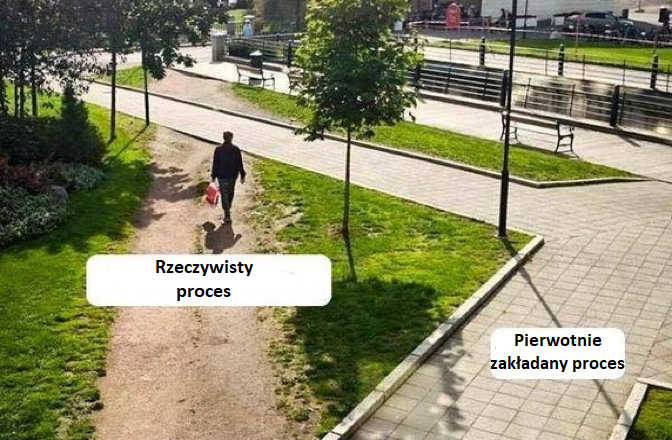
\includegraphics[scale=0.5]{model-vs-real.png}}
	\caption{\label{fig:subcaption_example}Proces rzeczywisty i pierwotnie zakładany}
\end{figure}

Celem automatycznego odkrywania procesów biznesowych jest zaprojektowanie funkcji - algorytmu, która przekształci dane z dziennika zdarzeń w model procesu \cite{pm-book}. Istnieje wiele algorytmów do odkrywania procesów biznesowych. Wśród najpopularniejszych można wymienić:
\begin{itemize}
  \item[•] Alpha algorithm \cite{alpha-algorithm}
  \item[•] The ILP Miner \cite{ILP-miner}
  \item[•] Heuristic Miner \cite{heuristics-miner}
  \item[•] Multi-phase Miner \cite{multi-phase-miner}
  \item[•] Inductive Miner \cite{inductive-miner}
\end{itemize}

Istnieją 4 powszechnie używane kryteria do określanie jak dobry jest otrzymany model. Są to:
\begin{itemize}
  \item[•] odwzorowanie (\textit{eng. fitness}) - zgodność modelu z dziennikiem zdarzeń
  \item[•] prostota (\textit{eng. simplicity}) - złożoność i łatwość zrozumienia modelu.
  \item[•] precyzja (\textit{eng. precision}) - brak zachowań niezwiązanych z logiem, a możliwych w modelu
  \item[•] generalizacja (\textit{eng. genralization}) - odzwierciedlenie w modelu prawdopodobnych aktywności, mimo że nie znajdują się one w logu.
\end{itemize}
Koniecznym jest znalezienie balansu między nimi, gdyż często starając się poprawiać model pod kontem jednego kryterium, pogorszy się on pod względem innych. Powstało wiele metryk przedstawiających te kryteria za pomocą wzorów matematycznych \cite{conf-propositions} \cite{Blum2015MetricsIP}.
Bardziej szczegółowo wybór metryk omówiono w sekcji \ref{sec:metryki}

Wśród istniejących algorytmów mogą pojawić się problemy ze współbieżnością, możliwością pomijania aktywności, czy reprezentowania duplikatów, nie radzeniem sobie z zakłócenia w logu,  tworzeniem zbyt skomplikowanych modeli, czy z odwzorowaniem niektórych zachowań. Modele stworzone mogą mieć zła strukturę Oparte na directly follows graphs przez co problemem może być kiedy log jest niekompletny.
Wciąż nie istnieje algorytm idealny, a te wymienione wyżej posiadają wady. Tworzą modele, które nie są spójne strukturalnie, czyli 
Algorytmy genetyczne do automatycznego odkrywania procesów biznesowych mogą być odpowiedzią na te problemy. Takie podejście pozwala na wyeliminowanie część problemów często dotyczących innych metod.  Ponadto każdy algorytm ma swoje ograniczenia a algorytmy genetyczne pozwalają na pełną dowolność
Pozwala na duża zdolność manipulacji, dobierania parametrów do tego co chcemy, wymyślania nowych. Można dodać tyle i takich metryk jakie chcemy, ustawić sobie różne wartości. Algorytmy klasyczne mają problem z uzyskanie dobrych rezultatów dla wszystkich metryk i nie posiadają możliwości zmiany parametrów startowych.

%---------------------------------------------------------------------------

\section{Ewolucja genetyczna}
\label{sec:ewolucjaGenetyczne}
\subsection{Algorytmy genetyczne}
\cite{ryan_collins_neill_1998}
Algorytmy genetyczne są inspirowaną selekcją naturalną  heurystyką, która używa znanych z ewolucji biologicznej operacji jak mutacja, selekcja czy krzyżowanie do rozwiązywania problemów wyszukiwania i optymizacji. Ich ideą jest zaproponowanie metody przeszukiwania przestrzeni losowy rozwiązań w celu wyszukania najlepszych z nich. Pierwszy raz zostały zaproponowane w \cite{10.5555/138936}.

Sposób działania algorytmów genetyczny polega na stworzeniu populacji losowych rozwiązań zwanych genotypami lub chromosomami, które kodowane są za pomocą licz całkowitych i zapisywane ww tablicy jednowymiarowej. Następnie dla każdego elementu populacji obliczana jest funkcja dopasowania (\textit{eng. fitness function}) pozwalająca ocenić jak dobre jest wygenerowane rozwiązanie. Po sklasyfikowaniu rozwiązań generujemy nową populację mutując lub krzyżując głownie choć nie tylko najlepsze chromosomy. Proces ten jest powtarzany do momentu otrzymania satysfakcjonującego rozwiązania.  

Utrzymywanie populacji rozwiązań fajna sprawa i pozwala na szerze zbiór rozwiązań.
Selekcja:
Selekcja proporcjonalna - wybieramy losowo rozwiązania z puli wszystkich rozwiązań z warunkiem, że rozwiązania z największą wartością metryk mają największą szansę na bycie zachowanymi w populacji. Jest to najpopularniejsza metoda selekcji i najczęściej umożliwiająca najszybsze znalezienie rozwiązania. Pozwala na elityzm, czyli zachowanie części najlepszych genotypów w przyszłej populacji.

Selekcja turniejowa - wybieramy podzbiór ze zbioru rozwiązań i zachowujemy w przyszłej najlepsze rozwiązanie z tego podzbioru.
Rozwiązanie to pozwala na duży wpływ na presję genetyczną - zwiększając wielkość podzbioru ograniczamy szansę na wybór z niską wartością metryk.  Jest to także metoda, która łatwe zrównoleglenie.

Krzyżowanie - :
Krzyżowanie punktowe - spośród dwóch genotypów losowo wybieramy jeden punkt, następnie tworzymy dwa nowe genotypy pierwszy z chromosomów na prawo od punktu w pierwszym genotypie i na lewo w genotypie drugim oraz drugi z dwóch pozostałych.

Krzyżowanie dwupunktowe - spośród dwóch genotypów losowo wybieramy dwa punkty, następnie część pomiędzy tymi punktami jest zamieniana pomiędzy genotypami.

Krzyżowanie n-punktowe - uogólnienie powyższych krzyżowań dla n punktów.

Krzyżowanie zamiana w drzewie - genotyp może być reprezentowany jako drzewo, w tej metodzie zamieniamy ze sobą dwa poddrzewa, tworzone są tylko prawidłowe rozwiązania, jednak jest to metoda wymagająca większej ilości obliczeń. 


Mutacja:
Mutacja punkowa - dowolna wartość w tablicy zostaje zmieniona na inną losową wartość. Pozostałe produkcje pozostają niezmienione.

Mutacja zamiana w drzewie - genotyp może być reprezentowany jako drzewo, w tej metodzie tworzone jest nowe poddrzewo, przy tej metodzie tworzone są tylko prawidłowe rozwiązania, jednak jest to metoda wymagająca większej ilości obliczeń. 

Algorytmy genetyczne w praktyce

 
  
\subsection{Ewolucja genetyczna a inne algorytmy uczenia maszynowego}
Algorytmy genetyczne pozwalają przeszukać najszerszą przestrzeń rozwiązań. Pozwalają na znajdowanie nieoczywistych rozwiązań.  
Inna heurystyką, która używa losowo rozwiązuje problem jest simulated annealing. Algorytm genetyczny jest łatwy w zrównogleniu i pozwala znaleźć globalne rozwiązanie.
Sieci neuronewe:
Pula rozwiązań zamiast jednego rozwiązywania. Szersze przeszukiwanie rozwiązań. 

Obejrzeć filmik na mlst.
\subsection{Ewolucja gramatyczna}
Ewoluuje gramatykę za pomocą metod ewolucji genetycznej w celu znalezienia programu, który najlepiej rozwiązuje problem.
Podejście to zostało zaproponowane w \cite{ryan_collins_neill_1998}. 

%---------------------------------------------------------------------------

\section{Gramatyka}
\label{sec:gramatyka}
\subsection{BNF}

Gramtyka G=(N,$\Sigma$,P,S) - 


Gramatyka bezkontekstowa - 


Backus-Naur from jest notacją używaną do kodowaniu gramatyk bezkontekstowych. Symbole używane w BNF to:



\subsection{Tworzenie gramatyki pod kątem ewolucji}

W celu ograniczenia niepotrzebnych obliczeń gramatyka powinna tworzyć jak najmniej niewłaściwych rozwiązań. 
Tworząc gramatykę pod kątem wykorzystania jej w procesie ewolucji ważne jest, żeby ilość produkcji jak najlepiej odzwierciedlała jak często chcemy uzyskać dany stan.
Stosując operator mutacji możemy uzyskać genotypy, które nie należą do języka, czyli nie są właściwym rozwiązaniami. Żeby ograniczyć zbędne obliczenia gramatyka powinna minimalizować szansę na to, że zamieniając produkcję na dowolną inną dostępną dla danego symbolu produkcję uzyskamy słowo które nie należy do języka.
Przykład:
a+b
<e> = aSe | b
<S> = + | -

<e> = aee | b | + | -

Produkcja 1:

<e> -> aSe -> a+e -> a+b
Produkcja 2:
<e> -> aee -> a+e -> a+b

Jeśli w kroku a+e zajdzie mutacja, może uzyskać gramatykę np. a+-, która nie należy do języka, dlatego pierwsza gramatyka jest lepsza.


%---------------------------------------------------------------------------

\section{Metryki}
\label{sec:metryki}

\subsection{Metryki a funkcja dopasowania}

Dobra funkcja dopasowania powinna spełniać kilka założeń, których nie wzięto pod uwagę tworząc metryki. 


Ostatecznie funkcja dopasowania w naszym algorytmie jest średnią ważoną metryk, gdzie użytkownik może określić z jakimi waga wziąć pod uwagę poszczególnych przystosowanych metryk. Oprócz tego dodano kolejną metrykę złożoność.

Ponadto wszystkie metryki powinny być przeskalowane jeśli to konieczne do przedziału od 0 do 1, co jest standardem i sprawia, że łatwiej je porównywać i na nich operować.

\subsection{Dodatkowa metryka - złożoność}
Dodatkowa metryka nie jest potrzebna, zawiera redundantne informacje, jednak istnieją teoretyczne przesłanki, że powinna wpłynąć pozytywnie na rozwiązania znajdowane przez algorytm. 
Ideą jest promowanie rozwiązywania prostych problemów w prosty sposób. Chcemy unikać lokalnych maksimów np. sytuacji, w której znajdziemy model, który   \newline
\subsection{Metryki - szczegóły}

\subsubsection{Prostota}
Najprostsza z metryk. Celem jest zmniejszenie skomplikowania. Głównym czynnikiem wpływającym na skomplikowanie jest ilość aktywności w modelu. Idealna jest sytuacja, w której model ma tyle samo aktywności ile unikalnych aktywności jest w dzienniku zdarzeń. To nie zawsze jest możliwe, jednak chcąc otrzymać maksymalnie czytelny model powinniśmy do tego dążyć. Stąd też metryk wybrana skupia się na dwóch czynnikach, czyli ilości duplikatów w modelu i ilości brakujących wartości w modelu. Oczywiście znaczenie ma wielkość modelu, dlatego wartości tego  musimy odnieść do ilości wszystkich zdarzeń w logu i modelu. Ostatecznie metrykę wyrażono wzorem: \newline
$M_{pro} = 1 - \frac{ilosc\ duplikatow\ w\ modelu\ +\ ilosc\ brakujacych\ zdarzen\ w\ modelu}{ilosc\ unikalnych\ zdarzen\ w\ logu\ +\ ilosc\ zdarzen\ w\ modelu}$
\subsubsection{Odwzorowanie}
Jest to najbardziej kosztowna obliczeniowo metryka. Pozostałe metryki obliczane są na podstawie tej metryki. Ważnym jest, żeby liczyć to częściowa, a sama metryka, żeby była maksymalnie wrażliwa na zmiany. Można by zastosować prostą metrykę zero-jedynkową, sprawdzającą czy model zgadza się z wariantem logu czy nie, jednak szczególnie w przypadku algorytmu genetycznego nie sprawdzalibyśmy jak bardzo zbliżamy się do celu i praktycznie opieralibyśmy się na losowaniu dopóki nie trafimy. Przy procesie z wieloma aktywnością niezgadzających się kilka kreatywności nie stworzyć dużego błędu, gdzie model zero-jedynkowy zrobiłby to, dlatego podniesiono do potęgi 4 , żeby zrobić metrykę bardziej wrażliwą na zmiany. Ostatecznie metrykę wyrażono wzorem: \newline
$M_o = (1 - \sum_{procesy\ w\ logu} \frac{blad\ odwzorowania\ logu\ w\ modelu}{minimalna\ długosc\ sciezki\ w\ modelu\ +\ długosc\ sciezki\ w\ logu})^4$
\subsubsection{Precyzja}
Unikanie niewystarczającego dopasowania (\textit{eng. underfitting}). Chcemy uniknąć tworzenia modeli, w której możliwe są dowolne zachowania. Można by osiągnąć maksymalne wartości pozostałych metryk tworząc jednak bramkę or zawierającą wszystkie aktywności, jednak oczywistym jest, że nie jest to model, które oddaje rzeczywistość. We wzorze skupiono się na ilości osiągalnych zdarzeń następujących po danej aktywności, możliwych w modelu. Chcemy żeby poszczególne aktywności mogły być tylko następowane przez te które naprawdę są po nich. Do potęgi 1/3, bo oryginalna metryka zienia się zbyt łatwo przez co jest nieproporcjonalna do zmian innych metryk i łatwo wpaść w lokalne maksimum, gdzie każda mała zmiana będzie wpływać na ogromną zmianę w metryce.  Ostatecznie metrykę wyrażono wzorem: \newline
$M_{pre} = (1 - \sum_{zdarzenia\ w\ modelu} \frac{ilosc\ osiagalnych\ zdarzen\ w\ modelu - ilosc\ osiagalnych\ zdarzen\ w\ logu}{ilosc\ osiagalnych\ zdarzen\ w\ modelu})^{\frac{1}{3}} $
\subsubsection{Generalizacja}
Unikanie nadmiernego dopasowania (\textit{eng. overfitting})
W pierwszej chwili może wydawać się przeciwieństwem precyzji, dobrym przykładem żeby to zwizualizować jest plama albo to z przetwarzania obrazów, chcemy wypełnić zagłębienia jednocześnie nie pozwalając na rozszerzenie. Można to osiągnąć poprzez wzięcie średniej ważonej liczby przejścia w logu przez dane zdarzenie, co sprawia, że wciąż zachowujemy ścieżki, które są często odwiedzane przez inne warianty, mimo że pozwalają na zachowanie niewidoczne w dzienniku zdarzeń, nie pozwalając na na tworzenie ścieżek, które nie pokrywają się z żadnymi ścieżkami. Wzięto także pierwiastek, gdyż od pewnego wykonywanie ścieżki wielokrotnie nie jest tak cenne jak wykonywanie jej, bo już wiemy, że jest ona ok. Metrykę zapożyczono z \cite{qd-in-discovery}. Ostatecznie metrykę wyrażono wzorem: \newline
$M_g = 1 - \frac{\sum_{zdarzenia\ w\ modelu} \frac{1}{\sqrt{ilosc\ wystapien\ zdarzenia}}}{ilosc\ zdarzen\ w\ logu} $
\subsubsection{Złożoność}
Postanowiono powiązać złożoność z odwzorowaniem, czyli kiedy odwzorowanie rośnie pozwalamy na tworzenie bardziej skomplikowanego modelu. Złożoność jest wyrażana jako ilość możliwych ścieżek w modelu. Jako, że np. dla bramki I jest to n! zauważamy, że złożoność rośnie niewspółmiernie szybciej do odwzorowania, dlatego pierwiastek ze złożoności. Ostatecznie metrykę wyrażono wzorem: \newline
$M_z = 1 - \frac{1}{\sqrt{1 - odwzorowanie\ *\ \sqrt{zlozonosc\ modelu}}} $

\subsection{Obliczanie metryk}
W sekcji \ref{sec:event_logs} przedstawiono przykład dziennika zdarzeń i warianty procesu obliczone dla niego. Weźmy pod uwagę model - na czerwono zaznaczono ilość wykonań danej aktywności:

\begin{figure}[h]
	\centering{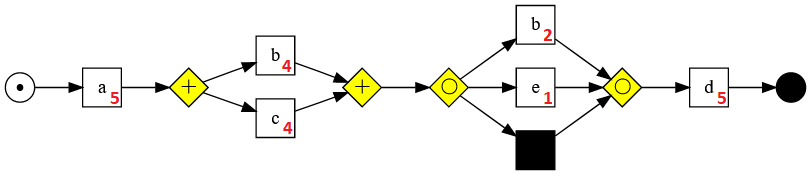
\includegraphics[scale=0.5]{model-metrics.png}}
	\caption{\label{fig:complicated_business_process_2}Model, dla którego obliczane są metryki}
\end{figure}

i obliczmy dla niego metryki.

$M_{pro} = 1 - \frac{1\ +\ 1}{6\ +\ 6} = 0.8333$

$Odwzorowanie = (1 - \sum_{ilosc\ procesow\ w\ logu} \frac{blad\ odwzorowania\ logu\ w\ modelu}{minimalna\ długosc\ sciezki\ w\ modelu\ +\ długosc\ sciezki\ w\ logu})^4$

$M_o = (1 - \sum_{ilosc\ procesow\ w\ logu} \frac{blad\ odwzorowania\ logu\ w\ modelu}{minimalna\ długosc\ sciezki\ w\ modelu\ +\ długosc\ sciezki\ w\ logu})^4$

$M_{pre} = (1 - \sum_{ilosc\ zdarzen\ w\ modelu} \frac{ilosc\ osiagalnych\ zdarzen\ w\ modelu - ilosc\ osiagalnych\ zdarzen\ w\ logu}{ilosc\ osiagalnych\ zdarzen\ w\ modelu})^{\frac{1}{3}} $

$M_g = 1 - \frac{(\frac{1}{\sqrt{5}}\ +\ \frac{1}{\sqrt{4}}\ +\ \frac{1}{\sqrt{4}}\ +\ \frac{1}{\sqrt{2}}\ +\ \frac{1}{\sqrt{1}}\ +\ \frac{1}{\sqrt{5}})}{6} = 0.3997$
\newline Pewną słabością tej metryki jest to, że wpływa na nią rozmiar dziennika zdarzeń. Jeśli ilość rekordów jest mała, jak w powyższym przykładzie, to generalizacja będzie słaba. Starając się znaleźć najlepszy model używamy zawsze tego samo logu, więc nie wpływa to na prawidłowość rozwiązania. \newline
$M_z = 1 - \frac{1}{\sqrt{1 - odwzorowanie\ *\ \sqrt{zlozonosc\ modelu}}} $